\documentclass[laboratorio]{guia}

\def \practnum {7} 
\def \practica {Ondas ac\'usticas}
% \def \practica {Ondas ac\'usticas en un tubo}

\def \materia {Laboratorio de F\'\i sica II para Qu\'\i micos}
\def \periodo {2do. Cuatrimestre de 2015}
\def \catedra {Pablo Cobelli}
\def \website {http://materias.df.uba.ar/f2qa2015c2}
 
\usepackage{graphics}
\usepackage{amsmath}
\usepackage{amsfonts}
\usepackage{graphicx}
\usepackage{float}
\usepackage{wrapfig}
\usepackage{subfigure}
\usepackage{bm}
\usepackage{grffile}
\usepackage{color}
\usepackage{framed}
\usepackage[utf8]{inputenc}
\usepackage[T1]{fontenc}
\usepackage{lmodern}
\usepackage{circuitikz}
\usepackage[spanish]{babel}
\usepackage{babelbib}
\selectbiblanguage{spanish}

 

%----------------------------------------------------------
% Agrega al path de figuras el subdirectorio con el mismo
%     nombre que el archivo principal del proyecto
\graphicspath{{./\jobname/}}

%----------------------------------------------------------
% Definicion del entorno 'sabermas'
\makeatletter
\definecolor{shadecolor}{rgb}{0.89,0.91,0.94}
\newenvironment{sabermas}[1]{%
\vfill
\begin{shaded}
  \begin{center}
  {\textsection{Para saber m\'as}}
  \end{center}
  #1
\sf } 
{%
\end{shaded}%
}
\makeatother

%----------------------------------------------------------
% Definicion del entorno 'problema'
\newcounter{ContadorProblema}
\setcounter{ContadorProblema}{0}
\newcounter{TieneFiguraAsociada}
\setcounter{TieneFiguraAsociada}{0}
\newcounter{UbicacionFigura}
\setcounter{UbicacionFigura}{0}

\newenvironment{problema}[2][]
{%
    \ifx\relax#1\relax%
        \setcounter{TieneFiguraAsociada}{0}
        \else
        \setcounter{TieneFiguraAsociada}{1}
    \fi
    \def \archivofigura {#1}
    % 
    \refstepcounter{ContadorProblema}
    \noindent%
    \ifnum\value{TieneFiguraAsociada} < 1%
        {\sffamily \bfseries Problema \arabic{ContadorProblema}.}
        %{\sc {#1}}%
        \par\nobreak\par\nobreak%
        \medskip 
    \else
        % Va con figura; resta determinar de que lado.
        \ifnum\value{UbicacionFigura} < 1
            % Poner la figura del lado derecho
            \begin{minipage}{12.25cm}
            {\sffamily \bfseries Problema \arabic{ContadorProblema}.}
            %{\sc {#1}}%
            \par\nobreak\par\nobreak%
            \medskip 
        \else
            % Poner la figura del lado izquierdo
            \begin{minipage}{4.5cm}
                \centering
                \includegraphics[width=4.5cm]{\archivofigura}
                {\footnotesize {\sffamily Esquema asociado al 
                problema \arabic{ContadorProblema}}.}
            \end{minipage}\hfill%
            \begin{minipage}{12.25cm}
                {\sffamily \bfseries Problema \arabic{ContadorProblema}.}
                %{\sc {#1}}%
                \par\nobreak\par\nobreak%
                \medskip 
        \fi
    \fi
}
{%
    \ifnum\value{TieneFiguraAsociada} < 1%
        % \par \bigskip \vskip 0.3cm
    \else
        % Va con figura; resta determinar de que lado.
        \ifnum\value{UbicacionFigura} < 1
            % Poner la figura del lado derecho
            \end{minipage}\hfill%
            \begin{minipage}{4.5cm}
                \centering
                \includegraphics[width=4.5cm]{\archivofigura}
                {\footnotesize {\sffamily Esquema asociado al 
                problema \arabic{ContadorProblema}}.}
            \end{minipage}
        \else
            % Poner la figura del lado izquierdo
            \end{minipage}%
        \fi
    \fi
    \setcounter{TieneFiguraAsociada}{0}
    \par \bigskip \vskip 0.3cm
    % Permutamos el valor de la ubicacion
    \ifnum\value{UbicacionFigura} < 1
        \setcounter{UbicacionFigura}{1}
    \else
        \setcounter{UbicacionFigura}{0}
    \fi
}

%----------------------------------------------------------
% Definicion/Redefinicion de estilos
\renewcommand{\vec}[1]{\ensuremath{\mathbf{#1}}}



\hyphenation{ coe-fi-cien-tes coe-fi-cien-te au-to-va-lor
              au-to-va-lo-res co-rres-pon-der pro-ble-ma 
              cual-quie-ra po-la-ri-za-cio-nes }

\graphicspath{{./acusticas/}}

\begin{document} 
\objetivo{%
  Realizar un estudio experimental de ondas acústicas en tubos; en el cuál se determinen experimentalmente las frecuencias de resonancia y la velocidad de propagación del sonido.
  \tematicas{ondas estacionarias, ondas acústicas, modos normales, frecuencias características, velocidad de propagación del sonido en aire.}
  }
\maketitle

\section{Tubo de Kundt}
El dispositivo experimental propuesto para el desarrollo de esta experiencia que recibe el nombre de su inventor, el físico alemán August Kundt.
\begin{figure}[htb]
    \centering
    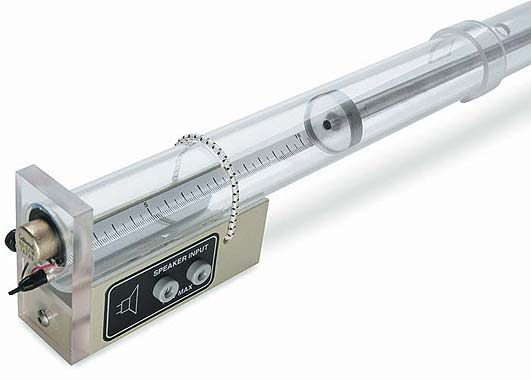
\includegraphics[width=0.4\textwidth]{pascoKundt}
    % 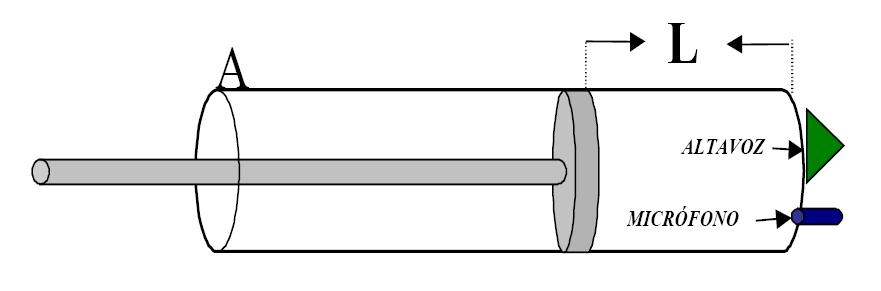
\includegraphics[width=0.5\textwidth]{Tubo_kundt_WikiCommons.jpeg}
    % 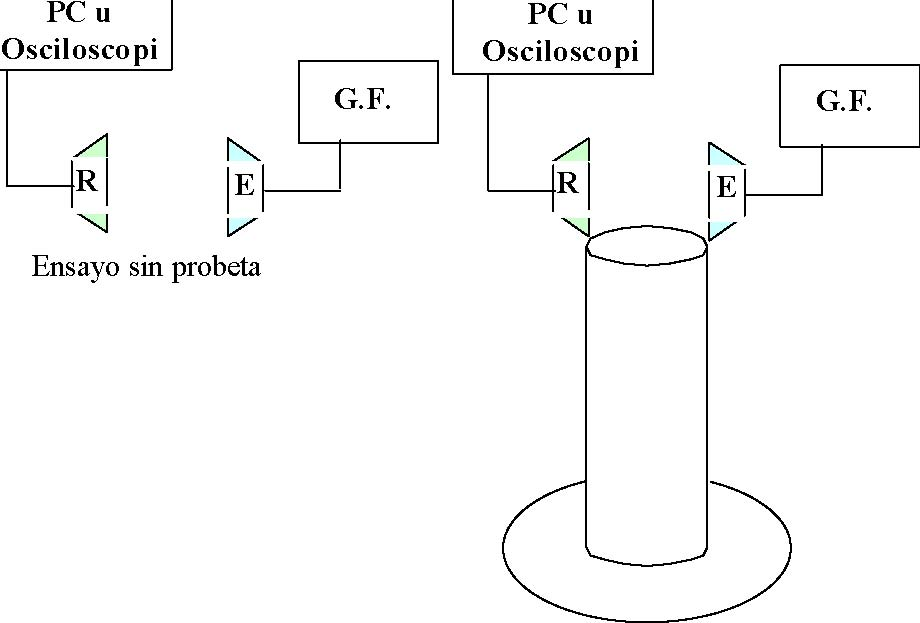
\includegraphics[width=8.5cm]{LG08--000.png}
    \caption{Tubo de Kundt del fabricante Pasco utilizado en el laboratorio de ondas del DF.}
    \label{fig:1}
\end{figure}
El elemento central del dispositivo es un tubo de acrílico transparente de sección circular, como se muestra en la figura \ref{fig:1}.
En un extremo del mismo un parlante mueve su membrana en función de la señal eléctrica que se le alimente.
La membrana impulsa el desplazamiento de las vecinas moléculas del aire.
Esto da lugar a una diferencia local de la presión respecto a la ambiente \(\delta p\).
Se genera así una onda de \(\delta p\) que se desplaza hacia el otro extremo del tubo, que de estar abierto presenta una \(\delta p = 0\).

Como alternativa a esta condición de \emph{extremo abierto}, puede limitarse la longitud que recorre la onda \(L\) ubicando un ``tapón'' en el interior del tubo.
El ``tapón'' impone un limitante al desplazamiento perpendicular a su superficie de las moléculas de aire.
En otras palabras, las moléculas ``chocan'' contra él, lo que produce que en su superficie se observe un máximo de \(\delta p\) (vientre de la onda) lo que da lugar a la llamada condición de \emph{extremo cerrado}.

Un micrófono puede posicionarse en cualquier posición entre parlante y el extremo, sea abierto o cerrado.
El micrófono opera como un parlante en inversa.
La señal que entrega es en función del desplazamiento de las moléculas de aire.
Así que cuando esta sea máxima, se está sensando un mínimo de \(\delta p\), es decir un nodo.
El micrófono se conecta a una etapa de amplificación lo que permite medir su señal con buena relación señal ruido en un osciloscopio (o, en su defecto, a un sistema de adquisición de datos asistidos por computadora). 

Una cinta métrica pegada a la cara interna del tubo permite medir las posiciones del ``tapón'' y micrófono respecto al parlante.
Los parámetros controlables son entonces: \(f\) del sonido, \(L\) de la cavidad y el punto en que se mide con el micrófono.


\subsection{Extremo cerrado}
En la idealización de tubo semicerrado la onda viajera emitida por el parlante, en \(x=0\), rebota con en el ``tapón'', en \(x=L\).
En determinadas frecuencias la rebotada refuerza (interferencia constructiva) la original dando lugar a una onda estacionaria.
Esta condición se cumple solo para las frecuencias llamadas de \textbf{resonancia}
\begin{equation}
  f(n)= \frac{v}{\lambda (n)},  
  \label{eq:frecuencialambda}
\end{equation}
donde \(v\) es la velocidad del sonido.

La condiciones a cumplir por la onda estacionaria son \(\delta p|_{x=0}= \delta p|_{x=L}=0\) por tanto las longitudes de onda permitidas son 
\begin{equation}
  \lambda_\text{abierto-cerrado}= \frac{4 L}{2 n+1}, \, n \in \mathbb{N}_0.
\end{equation}


\subsection{Extremo abierto}
Si obviamos el tapón aún se produce un rebote en el extremo abierto.
La onda ``rebota'' en respuesta a la diferencia de ``impedancia'' que se le presenta a la perturbación de la presión al pasar del confinamiento del tubo al ambiente abierto.

En tal caso las condiciones a cumplir por la onda estacionaria son \(\delta p|_{x=0}=0\) y \(\pdv{\delta p}{x}|_{x=L}=0\), donde \(L\) indica ahora el extremo abierto del tubo.
Esto hace que las longitudes de ondas permitidas para tal caso sean
\begin{equation}
  \lambda_\text{abierto-abierto}= \frac{2 L}{n+1}, \, n \in \mathbb{N}_0.
\end{equation}



\section{Desarrollo de la experiencia}

\subsection{Tubo abierto}
% Retire el ``tapón'' para tener la condición abierto-abierto, y alimente una señal sinusoidal al parlante.
% Establezca con el ``tapón'' una \(L\) arbitaria y alimente una señal al parlante.
Cuando el parlante impulsa el desplazamiento de las moléculas del aire estas no encuentran mas resistencia que las moléculas vecinas.
Como esta es mucho menor que la que ofrece una pared puede asumirse que allí \(\delta p\) no difiero mucho de un mínimo (nodo de la onda).

\textbullet\ 
Verifique moviendo el micrófono, y registrando la amplitud de la señal medida por este, si puede establecer en la proximidad del parlante un vientre o un nodo de \(\delta p\) que le sirva coma posición de referencia \(x=0\).
\textbf{Advertencia:} esta posición probablemente no sea la misma en cada uno de los modos.

\textbullet\ Dejando el micrófono quieto en alguna posición varíe la frecuencia del generador de funciones para determinar distintas frecuencias de resonancia.
Estas se manifestará por un pronunciado aumento de la amplitud de la señal medida.
En otras palabras, a las frecuencias de resonancia, para una dada amplitud de la excitación del emisor la respuesta del receptor (su amplitud) tiene un máximo relativo (dentro de un dado intervalo de frecuencia).
En estas condiciones determine por lo menos las primeras 5 resonancias en cada caso.
  Busque incluir la frecuencia fundamental (correspondiente a \(n=0\)) por debajo de la cual no se detectan otras resonancias.

\begin{itemize}
 \item Ahora que conoce las frecuencias de resonancia compare en una tabla la posición de los nodos que puede predecir a partir de conocer \(\lambda_n\) y los que encuentra barriendo el tubo con el micrófono.
  Note que la distancia entre nodos corresponde a \(\lambda_n\).
	Guarde registro de las que determina con el micrófono para cada uno de los \(n\) modos analizados.
    \item Grafique las frecuencias de resonancia del tubo en función del orden \(n\) de cada resonancia, es decir, el índice que identifica su aparición cuando se incrementa monótonamente la frecuencia.
\end{itemize}


\subsection{Dependencia con la longitud}
En esta segunda parte nos proponemos determinar la variación en la respuesta del sistema cuando se modifica la longitud del tubo, esto es utilizando el ``tapón'' para tener la condición abierto-cerrado.
Para ello, la propuesta consiste en repetir el mismo estudio precedente para \emph{al menos} dos longitudes \(L\) que serán menores que la del tubo, empleada en la primera parte.

En estas nuevas condiciones:
\begin{itemize}
    \item Determine las primeras cinco frecuencias de resonancia \(f_n\) del tubo.
		% Grafique el producto \(f_n L\) en función del orden \(n\), para todos los casos estudiados.
    % \item Suponiendo que en el tubo semicerrado caben exactamente \((2n+1)\) cuartos de longitudes de onda, trate de dar cuenta de sus resultados experimentales.
    \item Realice para cada una de las \(L\) ensayadas un gráfico de \(f_n L\) en función del orden \(n\).
\end{itemize}

\subsection{Velocidad del sonido}
Asumiendo que se cumplen las condiciones adiabáticas, que el aire tiene una humedad despreciable y por tanto está mayoritariamente compuesto por gases diatómicos (\isotope{N_2} y \isotope{O_2})
\[
	v_\mathrm{adiab.}= \sqrt{\frac{C_p}{C_v} \frac{P_0}{\rho_0}} \simeq \sqrt{1,4\frac{P_0}{\rho_0}},
\]
donde para el aire en CNPT, \(P_0=1\,\mathrm{atm}= \SI{101300}{\pascal}\) y \(\rho_0 = \SI{1,225}{\kilo\gram\over\cubic\metre}\), puede calcular un valor de referencia para la velocidad del sonido \(v\).

Con las mediciones que efectuó en los puntos anteriores y usando la relación (\ref{frencuencialambda}) debiera ser capaz de graficar \(f_n\) en función de \(1/\lambda_n\) y de verificarse la linealidad esperada obtener de la pendiente una estimación de \(v\).
Discuta y especule acerca de las posibles discrepancias entre uno y otro valor obtenido.

\subsubsection{Diámetro finito del tubo} 
Una consecuencia de tener un diámetro finito en el tubo es que su longitud efectiva es mayor que su longitud geométrica, ya que no se tiene una propagación de la onda estríctamente unidimensional.
Esto causa que el número de medias longitudes de onda que caben en dicha longitud efectiva \(L_\text{ef}\) satisfaga
\begin{equation*}
  L_\text{ef} = L + \alpha d = n \frac{\lambda_n}{2}.
\end{equation*}
¿Cómo afecta esta corrección sus conclusiones respecto de la velocidad de propagación del sonido en aire?
Tenga en cuenta que el valor de \(\alpha\) es del orden de 0.4 para un tubo semicerrado, y del orden de 0.8 para uno abierto.


%\subsection{Ancho espectral de las resonancias}
%Determine, para las resonancias encontradas en la primera parte, sus
%respectivos semianchos en el espacio de frecuencias. Estos se definen como las
%distancias (en frecuencia) en las que la amplitud cae a la mitad de su valor en
%resonancia.
%
%
%\subsection{Estudio en funci\'on de la posici\'on del detector}
%Para por lo menos 3 frecuencias de resonancia, estudie experimentalmente c\'omo
%var\'\i an la amplitud y la fase en funci\'on de la posici\'on del detector en
%el tubo. Grafique sus resultados. ?`Qu\'e puede concluir acerca de estos
%resultados? ?`Est\'an de acuerdo con la teor\'\i a propuesta? ?`C\'omo es la
%amplitud en los extremos del tubo? Concretamente: en los extremos abierto y
%cerrado, ?`hay nodos o extremos de amplitud? Explique sus resultados con
%argumentos f\'\i sicos.

\nocite{Alonso1998,Crawford1994}
\bibliographystyle{unsrt} 
\bibliography{Bibliografia}




\end{document}
